\documentclass{standalone}
\usepackage{tikz}
\usetikzlibrary{arrows}
\begin{document}
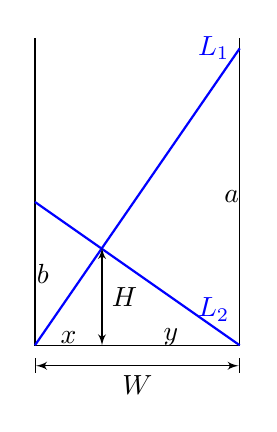
\begin{tikzpicture}[>=latex',scale=1.3]
\draw (0,3) -- (0,0) -- (2,0) -- (2,3);
\draw[blue, thick] (0,0) -- (2,2.9) node[left] {$L_1$};
\draw[blue, thick] (2,0) node[above left, yshift=5] {$L_2$} -- (0,1.4);
\draw[|<->|] (0,-.2) -- node[below] {$W$} (2,-.2);
\draw[<->] (.655,0) -- node[right] {$H$} (.655,.95);
\node[xshift=.1cm] at (0,.7) {$b$};
\node[xshift=-.1cm] at (2,1.45) {$a$};
\node[yshift=.1cm] at (.3275,0) {$x$};
\node[yshift=.1cm] at (1.3275,0) {$y$};

\end{tikzpicture}	
\end{document} 
